
\documentclass{standalone}
\usepackage{tikz} 
\usetikzlibrary{arrows}
\usetikzlibrary{shapes}
\usetikzlibrary{shapes.misc}

\begin{document}

\centering
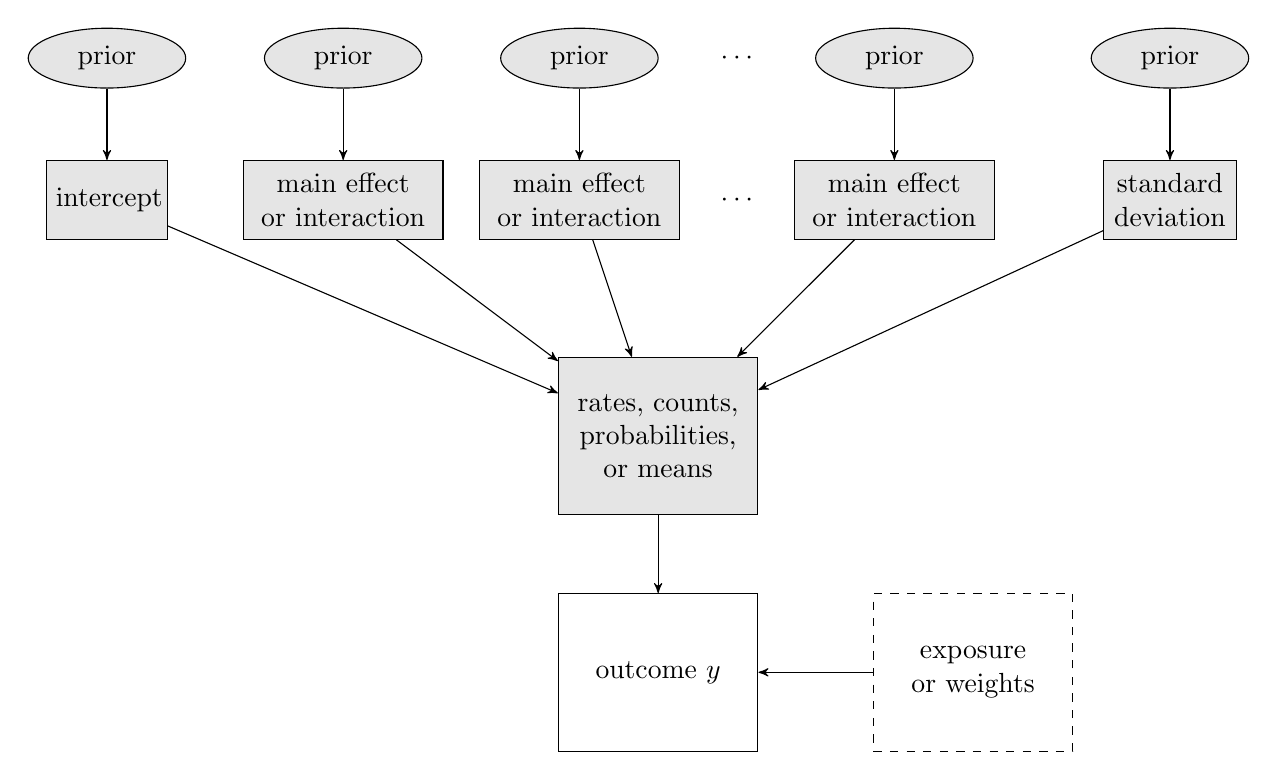
\begin{tikzpicture}
\tikzset{
   node distance = 3cm, >=stealth',
   array/.style = {rectangle, draw, minimum width = 2.3cm, text width = 2.3cm, align = center},
   big_array/.style = {array, minimum height = 2cm},
   big_array_obs/.style = {big_array},
   big_array_unobs/.style = {big_array, fill = black!10},
   small_array/.style = {array, minimum height = 1cm, fill = black!10},
   scalar/.style = {small_array, minimum width = 1.3cm, text width = 1.3cm},
   prior/.style = {ellipse, draw, fill = black!10, node distance = 1.8cm, minimum width = 2cm} 
}
  \node [big_array_obs] (y) [] {outcome $y$};
  \node [big_array_obs] (ew) [right of = y, dashed, xshift = 1cm] {exposure or weights}
        edge [->] (y);

  \node[big_array_unobs] (gamma) [above of = y] {rates, counts, probabilities, or means}
        edge [->] (y);

  \node[] (dots_effect) [above of = gamma, xshift = 1cm] {$\cdots$};
  \node[small_array] (effect_last) [right of = dots_effect, xshift = -1cm] {main effect or interaction}
        edge [->] (gamma);
  \node[small_array] (effect_second) [left of = dots_effect, xshift = 1cm] {main effect or interaction}
        edge [->] (gamma);
  \node[small_array] (effect_first) [left of = effect_second] {main effect or interaction}
        edge [->] (gamma);
  \node[scalar] (intercept) [left of = effect_first] {intercept}
        edge [->] (gamma);
  \node[scalar] (sd) [right of = effect_last, text width = 1.45cm, xshift = 0.5cm] {standard deviation}
        edge [->] (gamma);

  \node[prior] (prior_intercept) [above of = intercept] {prior}
       edge [->] (intercept);
  \node[prior] (prior_effect_first) [above of = effect_first] {prior}
       edge [->] (effect_first);
  \node[prior] (prior_effect_second) [above of = effect_second] {prior}
       edge [->] (effect_second);
  \node[] (dots_prior) [above of = dots_effect, node distance = 1.8cm] {$\cdots$};
  \node[prior] (prior_effect_last) [above of = effect_last] {prior}
       edge [->] (effect_last);
  \node[prior] (prior_sd) [above of = sd] {prior}
       edge [->] (sd);

\end{tikzpicture}

\end{document}